% !TEX root = main.tex
\section{Ativos e Passivos: A Base para a Prosperidade Financeira.}

\begin{frame}[c]\frametitle{Ativos}
  \textbf{O que são Ativos?}
  \begin{itemize}
    \item São todos os bens e recursos que você possui e que geram renda ou se valorizam com o tempo.
  \end{itemize}

  \textbf{Exemplos de Ativos:}
  \begin{itemize}
    \item Investimentos (Ações, títulos, fundos, etc.)
    \item Imóveis
    \item Seu próprio negócio ou fonte de renda
    \item Tudo aquilo que te gera renda.
  \end{itemize}
\end{frame}

\begin{frame}[c]\frametitle{Passivos}
  \textbf{O que são Passivos?}
  \begin{itemize}
    \item São todas as obrigações financeiras que você tem a pagar, ou seja, tudo que tira dinheiro do seu bolso.
  \end{itemize}

  \textbf{Exemplos de Passivos:}
  \begin{itemize}
    \item Dívidas (empréstimos, financiamento de carro, cartão de crédito)
    \item Contas fixas (aluguel, condomínio, luz, internet)
    \item Impostos e juros
    \item Tudo aquilo que te gera despesa.
  \end{itemize}
\end{frame}


\begin{frame}[c]\frametitle{O Fluxo do Dinheiro}
  \begin{center}
    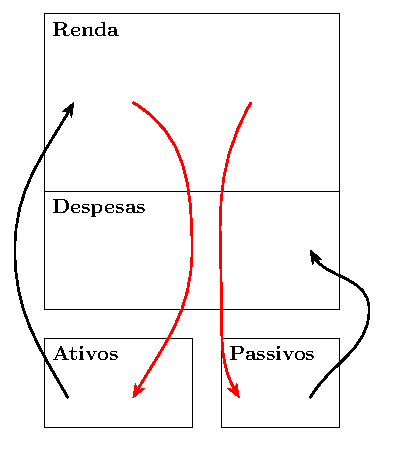
\includegraphics{../figuras/pai_rico}
  \end{center}
\end{frame}

\begin{frame}[c]\frametitle{O Impacto no Patrimônio}
  \begin{columns}
    \begin{column}{0.5\textwidth}
      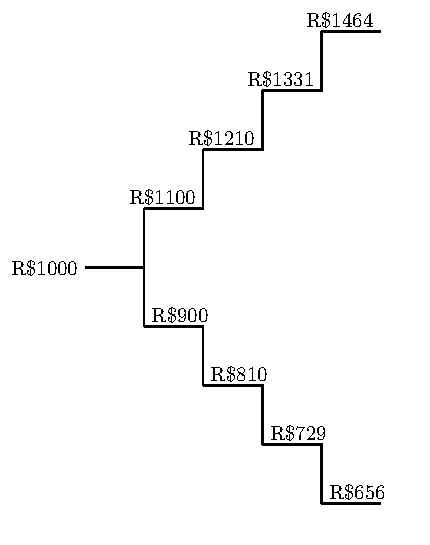
\includegraphics[width=\textwidth]{figuras/dobra4.pdf}
    \end{column}
    \begin{column}{0.5\textwidth}
      \centering
      \textbf{\large Ao final de 4 anos um ativo rendendo de 10\% a.a. vale mais que o dobro de um passivo que desvaloriza na mesma taxa.}
      % \begin{itemize}
      %   \item Taxa de juros anual de 10\% a.a.
      %   \item $\frac{\text{R\$ 1464}}{\text{R\$656}} = 2,23$.
      %   \item Tentar gerar renda extra.
      %   \item Não aumentar os gastos devido a aumento salarial.
      % \end{itemize}
    \end{column}
  \end{columns}
\end{frame}

\begin{frame}[c]\frametitle{Exemplo Prático: A Compra um Carro}
  \textbf{Patrimônio Inicial:} R\$120.000,00

  \begin{itemize}
    \item \textbf{Cenário 1:} Gasta R\$100.000,00 na compra de um carro e investe o restante.
    \item \textbf{Cenário 2:} Gasta R\$60.000,00 na compra de um carro e investe o restante.
    \item \textbf{Cenário 3:} Não compra o carro e investe os R\$120.000,00.
  \end{itemize}

  \textbf{Premissas:}
  \begin{itemize}
    \item Desvalorização do carro: 10\% ao ano.
    \item Custo de Oportunidade: 12\% ao ano (quanto o dinheiro rende investido).
  \end{itemize}
\end{frame}

\begin{frame}[c]\frametitle{Analisando o Cenário 1}
  \textbf{Decisão: Comprar carro de R\$100 mil e investir R\$20 mil}
  \begin{itemize}
    \item \textbf{Patrimônio Inicial:} R\$ 120.000,00
    \item \textbf{Carro (depreciação de 10\% a.a.)}: R\$ 100.000,00
    \item \textbf{Saldo Investido (rendimento de 12\% a.a.)}: R\$ 20.000,00
  \end{itemize}
  \begin{center}
    \begin{tabular}{|c|c|c|c|}
      \hline
      \textbf{Ano} & \textbf{Valor do Carro} & \textbf{Valor Investido} & \textbf{Patrimônio Total} \\
      \hline
      \textbf{0}   & R\$ 100.000,00          & R\$ 20.000,00            & R\$ 120.000,00            \\
      \textbf{1}   & R\$ 90.000,00           & R\$ 22.400,00            & R\$ 112.400,00 (-6,33\%)  \\
      \textbf{2}   & R\$ 81.000,00           & R\$ 25.088,00            & R\$ 106.088,00 (-5,62\%)  \\
      \textbf{3}   & R\$ 72.900,00           & R\$ 28.098,56            & R\$ 100.998,56 (-4,80\%)  \\
      \textbf{4}   & R\$ 65.610,00           & R\$ 31.470,39            & R\$ 97.080,39  (-3,88\%)  \\
      \textbf{5}   & R\$ 59.049,00           & R\$ 35.246,83            & R\$ 94.295,83  (-2,87\%)  \\
      \hline
    \end{tabular}
  \end{center}
\end{frame}

\begin{frame}[c]\frametitle{Analisando o Cenário 2}
  \textbf{Decisão: Comprar carro de R\$60.000,00 e investir R\$60.000,00}
  \begin{itemize}
    \item \textbf{Patrimônio Inicial:} R\$ 120.000,00
    \item \textbf{Carro (depreciação de 10\% a.a.)}: R\$ 60.000,00
    \item \textbf{Saldo Investido (rendimento de 12\% a.a.)}: R\$ 60.000,00
  \end{itemize}
  \begin{center}
    \begin{tabular}{|c|c|c|c|}
      \hline
      \textbf{Ano} & \textbf{Valor do Carro} & \textbf{Valor Investido} & \textbf{Patrimônio Total} \\
      \hline
      \textbf{0}   & R\$ 60.000,00           & R\$ 60.000,00            & R\$ 120.000,00            \\
      \textbf{1}   & R\$ 54.000,00           & R\$ 67.200,00            & R\$ 121.200,00 (+1,00\%)  \\
      \textbf{2}   & R\$ 48.600,00           & R\$ 75.264,00            & R\$ 123.864,00 (+2,20\%)  \\
      \textbf{3}   & R\$ 43.740,00           & R\$ 84.295,68            & R\$ 128.035,68 (+3,37\%)  \\
      \textbf{4}   & R\$ 39.366,00           & R\$ 94.411,16            & R\$ 133.777,16 (+4,48\%)  \\
      \textbf{5}   & R\$ 35.429,40           & R\$ 105.740,50           & R\$ 141.169,90 (+5,53\%)  \\
      \hline
    \end{tabular}
  \end{center}
\end{frame}

\begin{frame}[c]\frametitle{Patrimônio Ano a Ano nos 3 cenários}
  \begin{center}
    \begin{tabular}{|l|c|c|c|}
      \hline
      \textbf{Ano} & \textbf{Cenário 1} & \textbf{Cenário 2} & \textbf{Cenário 3} \\
      \hline
      \textbf{0}   & R\$ 120.000,00     & R\$ 120.000,00     & R\$ 120.000,00     \\
      \textbf{1}   & R\$ 112.400,00     & R\$ 121.200,00     & R\$ 134.400,00     \\
      \textbf{2}   & R\$ 106.088,00     & R\$ 123.864,00     & R\$ 150.528,00     \\
      \textbf{3}   & R\$ 100.998,56     & R\$ 128.035,68     & R\$ 168.591,36     \\
      \textbf{4}   & R\$ 97.080,39      & R\$ 133.777,16     & R\$ 188.822,32     \\
      \textbf{5}   & R\$ 94.295,83      & R\$ 141.169,90     & R\$ 211.481,00     \\
      \hline
    \end{tabular}
  \end{center}
\end{frame}


\begin{frame}[c]\frametitle{Retorno Final após 5 anos}
  \begin{tabular}{|l|c|c|c|}
    \hline
    \textbf{Cenário}   & \textbf{Patrimônio Final} & \textbf{Retorno Total (R\$)} & \textbf{Retorno Total (\%)} \\
    \hline
    \textbf{Cenário 1} & R\$ 94.295,83             & -R\$ 25.704,17               & -21,42\%                    \\
    \textbf{Cenário 2} & R\$ 141.169,90            & +R\$ 21.169,90               & +17,64\%                    \\
    \textbf{Cenário 3} & R\$ 211.481,00            & +R\$ 91.481,00               & +76,23\%                    \\
    \hline
  \end{tabular}
\end{frame}